\documentclass[a4paper]{article}

\input{style/ch_xelatex.tex}
\input{style/scala.tex}

%代码段设置
\lstset{numbers=left,
basicstyle=\tiny,
numberstyle=\tiny,
keywordstyle=\color{blue!70},
commentstyle=\color{red!50!green!50!blue!50},
frame=single, rulesepcolor=\color{red!20!green!20!blue!20},
escapeinside=``
}

\graphicspath{ {images/} }
\usepackage{ctex}
\usepackage{graphicx}
\usepackage{color,framed}%文本框
\usepackage{listings}
\usepackage{caption}
\usepackage{amssymb}
\usepackage{enumerate}
\usepackage{xcolor}
\usepackage{bm} 
\usepackage{lastpage}%获得总页数
\usepackage{fancyhdr}
\usepackage{tabularx}  
\usepackage{geometry}
\usepackage{minted}
\usepackage{graphics}
\usepackage{subfigure}
\usepackage{float}
\usepackage{pdfpages}
\usepackage{pgfplots}
\pgfplotsset{width=10cm,compat=1.9}
\usepackage{multirow}
\usepackage{footnote}
\usepackage{booktabs}
\pgfplotsset{compat=1.17} % 或者你当前安装的版本

%-----------------------伪代码------------------
\usepackage{algorithm}  
\usepackage{algorithmicx}  
\usepackage{algpseudocode}  
\floatname{algorithm}{Algorithm}  
\renewcommand{\algorithmicrequire}{\textbf{Input:}}  
\renewcommand{\algorithmicensure}{\textbf{Output:}} 
\usepackage{lipsum}  
\makeatletter
\newenvironment{breakablealgorithm}
  {% \begin{breakablealgorithm}
  \begin{center}
     \refstepcounter{algorithm}% New algorithm
     \hrule height.8pt depth0pt \kern2pt% \@fs@pre for \@fs@ruled
     \renewcommand{\caption}[2][\relax]{% Make a new \caption
      {\raggedright\textbf{\ALG@name~\thealgorithm} ##2\par}%
      \ifx\relax##1\relax % #1 is \relax
         \addcontentsline{loa}{algorithm}{\protect\numberline{\thealgorithm}##2}%
      \else % #1 is not \relax
         \addcontentsline{loa}{algorithm}{\protect\numberline{\thealgorithm}##1}%
      \fi
      \kern2pt\hrule\kern2pt
     }
  }{% \end{breakablealgorithm}
     \kern2pt\hrule\relax% \@fs@post for \@fs@ruled
  \end{center}
  }
\makeatother
%------------------------代码-------------------
\usepackage{xcolor} 
\usepackage{listings} 
\lstset{ 
breaklines,%自动换行
basicstyle=\small,
escapeinside=``,
keywordstyle=\color{ blue!70} \bfseries,
commentstyle=\color{red!50!green!50!blue!50},% 
stringstyle=\ttfamily,% 
extendedchars=false,% 
linewidth=\textwidth,% 
numbers=left,% 
numberstyle=\tiny \color{blue!50},% 
frame=trbl% 
rulesepcolor= \color{ red!20!green!20!blue!20} 
}

%-------------------------页面边距--------------
\geometry{a4paper,left=2.3cm,right=2.3cm,top=2.7cm,bottom=2.7cm}
%-------------------------页眉页脚--------------
\usepackage{fancyhdr}
\pagestyle{fancy}
\lhead{\kaishu \leftmark}
% \chead{}
\rhead{\kaishu 并行程序设计实验报告}%加粗\bfseries 
\lfoot{}
\cfoot{\thepage}
\rfoot{}
\renewcommand{\headrulewidth}{0.1pt}  
\renewcommand{\footrulewidth}{0pt}%去掉横线
\newcommand{\HRule}{\rule{\linewidth}{0.5mm}}%标题横线
\newcommand{\HRulegrossa}{\rule{\linewidth}{1.2mm}}
\setlength{\textfloatsep}{10mm}%设置图片的前后间距
%--------------------文档内容--------------------
% 允许浮动体占用页面的 80% (默认只有 70%)
\renewcommand{\topfraction}{.85}
\renewcommand{\bottomfraction}{.7}
\renewcommand{\textfraction}{.15}
\renewcommand{\floatpagefraction}{.66}
\renewcommand{\dbltopfraction}{.66}
\renewcommand{\dblfloatpagefraction}{.66}
\setcounter{topnumber}{9}
\setcounter{bottomnumber}{9}
\setcounter{totalnumber}{20}
\begin{document}
\renewcommand{\contentsname}{目\ 录}
\renewcommand{\appendixname}{附录}
\renewcommand{\appendixpagename}{附录}
\renewcommand{\refname}{参考文献} 
\renewcommand{\figurename}{图}
\renewcommand{\tablename}{表}
\renewcommand{\today}{\number\year 年 \number\month 月 \number\day 日}

%-------------------------封面----------------
\begin{titlepage}
    \begin{center}
    
\includegraphics[width=0.8\textwidth]{NKU.png}\\[1cm]
    \vspace{20mm}
		\textbf{\huge\textbf{\kaishu{计算机学院}}}\\[0.5cm]
		\textbf{\huge{\kaishu{并行程序设计实验报告}}}\\[2.3cm]
		\textbf{\Huge\textbf{\kaishu{作业二:体系结构及性能相关测试}}}

		\vspace{\fill}
    
    % \textbf{\Large \textbf{并行程序设计期末实验报告}}\\[0.8cm]
    % \HRule \\[0.9cm]
    % \HRule \\[2.0cm]
    \centering
    \textsc{\LARGE \kaishu{姓名\ :\ 罗雅淇}}\\[0.5cm]
    \textsc{\LARGE \kaishu{学号\ :\ 2313483}}\\[0.5cm]
    \textsc{\LARGE \kaishu{专业\ :\ 计算机科学与技术}}\\[0.5cm]
    
    \vfill
    {\Large 2026年3月28日}
    \end{center}
\end{titlepage}

\renewcommand {\thefigure}{\thesection{}.\arabic{figure}}%图片按章标号
\renewcommand{\figurename}{图}
\renewcommand{\contentsname}{目录}  
\cfoot{\thepage\ of \pageref{LastPage}}%当前页 of 总页数


% 生成目录
\clearpage
\tableofcontents
\newpage
\section{引言}
\subsection{实验概述}
在本实验中，我完成了矩阵向量内积和n个数求和两个实验的基础任务，分别实现了平凡算法和优化算法（Cache优化/超标量优化），并设计了多个规模的实验，通过高精度计时程序来测试性能。
进阶任务方面，我额外实现了循环展开和递归算法，完成了不同优化级别对性能的影响和浮点数精度对性能的影响这两个进阶任务的探索。最后我学习使用VTune作为Profiling工具，对两个实验都进行了更深入的性能分析。
\subsection{核心代码}
代码仓库地址：\href{https://github.com/lyaqiqi/NKU_Parallel_Programming_2026}{https://github.com/lyaqiqi/NKU\_Parallel\_Programming\_2026}
%--------------------------Title--------------------------------

\section{体系结构相关实验分析——cache 优化}
\subsection{实验要求}
给定一个 n × n 矩阵，计算每一列与给定向量的内积，考虑两种算法设计思路：逐列访问元素的平凡算法和 cache 优化算法，进行实验对比：
\begin{enumerate}
  \item 对两种思路的算法编程实现；
  \item 练习使用高精度计时测试程序执行时间，比较平凡算法和优化算法的性能。
\end{enumerate}

\subsection{算法设计}
\subsubsection{平凡算法}
设计思路为纯模拟思路，让 a 中的每一个元素和 b 中的每一列元素相乘，其中逐列访问 b 中元素，再将结果加到 sum 中。
\begin{minted}[mathescape,
               linenos,
               numbersep=5pt,
               gobble=2,
               frame=lines,
               framesep=2mm,
               highlightcolor=green!40]{c}
    void trivial_algorithm(long long n, const double* b, const double* a, double* sum) {
        if (n == 0) return;
        for (long long i = 0; i < n; i++) {
            sum[i] = 0.0;
            for (long long j = 0; j < n; j++) {
                // 按列遍历矩阵，导致内存跳跃访问
                sum[i] += b[j * n + i] * a[j];
            }}}
\end{minted}
\subsubsection{Cache 优化算法}
让 a 中的每一个元素和 b 中的每一行元素相乘，逐行访问 b 中元素，并且把局部结果加到 sum 中，当循环全部结束后才得到所有结果。cache 优化算法与 C++ 使用的行主存储模式相匹配，具有很好的空间局部性，令 cache 作用能够很好的发挥。
\begin{minted}[mathescape,
               linenos,
               numbersep=5pt,
               gobble=2,
               frame=lines,
               framesep=2mm,
               highlightcolor=green!40]{c}
    void optimized_algorithm(long long n, const double* b, const double* a, double* sum) {
        if (n == 0) return;
        for (long long i = 0; i < n; i++) {
            sum[i] = 0.0;
        }
        for (long long j = 0; j < n; j++) {
            for (long long i = 0; i < n; i++) {
                // 嵌套循环反转，按行连续遍历矩阵元素
                sum[i] += b[j * n + i] * a[j];
            }}}
\end{minted}
\subsection{实验过程}

实验在 x86 平台（Windows 11）上运行，使用 MinGW g++ 4.9.2 编译器，采用 \texttt{QueryPerformanceCounter} 进行高精度计时。

实验分为两个测试阶段。第一阶段（cache 优化效果测试）固定编译优化等级为 \texttt{-O2}，采用分段线性的矩阵规模设计：在 $n \in [16, 128]$ 和 $n \in [144, 512]$ 范围内以步进 16 密集采样，在 $n \in [576, 2048]$ 范围内以步进 64 采样，共 56 个规模点，以覆盖 L1、L2、L3 各 cache 层级的跨越边界。第二阶段（编译器优化等级测试）使用固定的 14 组 $\{n, \text{重复次数}\}$ 配置，对 \texttt{-O0} 至 \texttt{-O3} 四个等级分别测试。每组实验均进行预热后计时，并通过动态重复次数策略（小规模多次、大规模少次）保证总计时时长，减小误差。两种算法的输出结果在每次运行后进行一致性校验。

\subsection{性能分析}

\subsubsection{不同规模下的执行时间及Cache优化效果}
\begin{figure}[htbp]
    \centering
    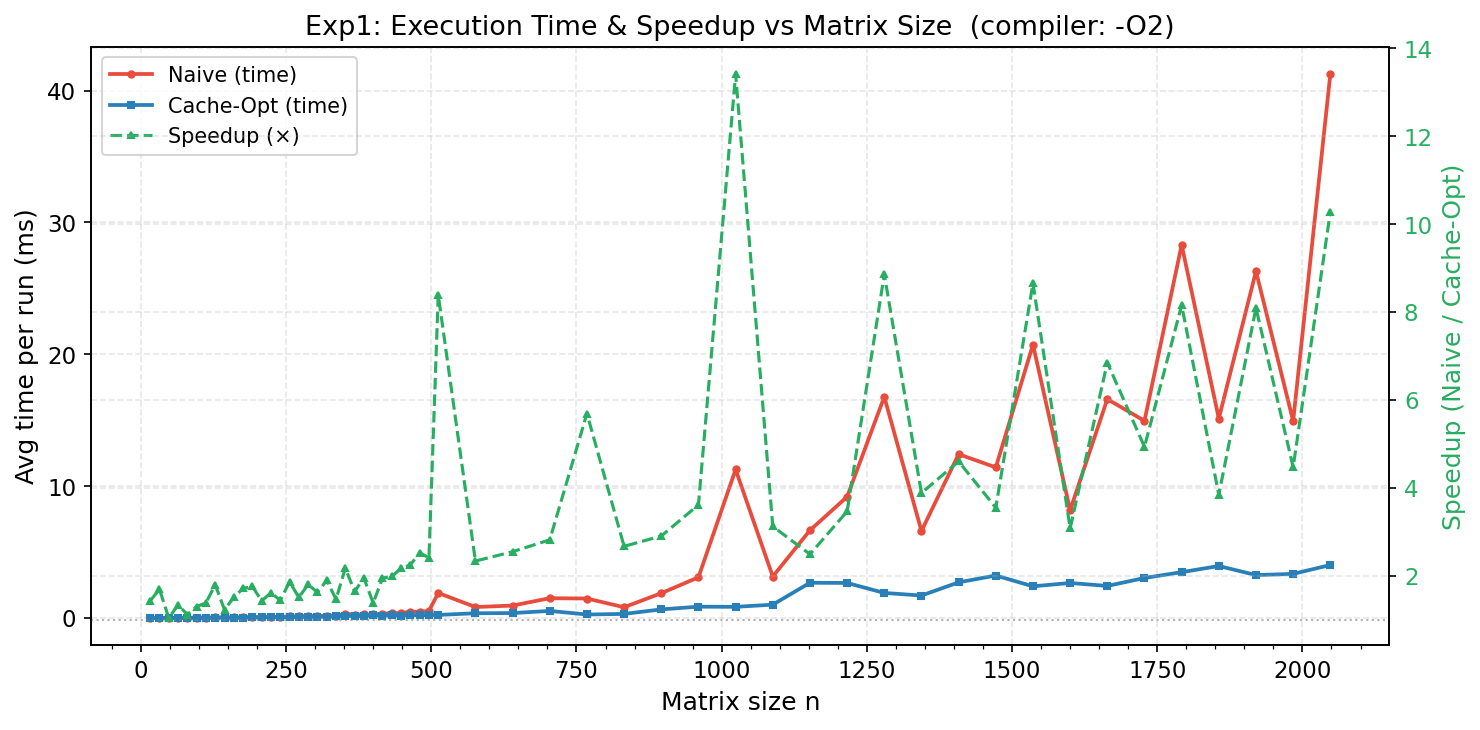
\includegraphics[width=0.8\textwidth]{fig/fig1_time_speedup.png}
    \caption{平凡算法和Cache优化算法在不同规模下的执行时间及加速比}
    \label{fig:cache}
\end{figure}
实验结果如图 \ref{fig:cache}所示。在小规模阶段（$n \lesssim 64$），矩阵数据量约为 $8n^2 \approx 32\text{KB}$，可完全装入 L1 cache，两种算法执行时间相当，加速比接近 1。随着 $n$ 增大至 L1 边界附近，平凡算法的列访问步长为 $n$，频繁触发 cache miss，执行时间快速上升；优化算法按行连续访问，cache 命中率高，执行时间增长平缓。

在 $n \approx 512$ 至 $1024$ 区间，加速比出现多次峰值，最高达约 14 倍，此时矩阵规模恰好跨越 L2 cache 边界，平凡算法对 L2、L3 的反复失效代价被充分暴露。$n > 1024$ 后，两种算法均超出 L3 cache 容量，优化算法的绝对优势趋于稳定（加速比维持在 8 至 10 倍），但加速比不再单调增长，受限于内存带宽上限。
\subsubsection{进阶任务：不同优化级别下的执行性能}

不同编译器优化等级对两种算法的影响如表所示。

\begin{table}[!ht]
\centering
\caption{不同编译器优化等级下的平均执行时间（ms/次）}
\label{tab:compiler_opt}
\resizebox{\textwidth}{!}{%
\begin{tabular}{r r | r r r r | r r r r}
\toprule
\multirow{2}{*}{$n$} & \multirow{2}{*}{重复次数} & \multicolumn{4}{c|}{平凡算法（Naive）} & \multicolumn{4}{c}{优化算法（Cache-Opt）} \\
 & & \texttt{-O0} & \texttt{-O1} & \texttt{-O2} & \texttt{-O3} & \texttt{-O0} & \texttt{-O1} & \texttt{-O2} & \texttt{-O3} \\
\midrule
10    & 10000 & 0.001309 & 0.000269 & 0.000156 & 0.000159 & 0.000468 & 0.000183 & 0.000143 & 0.000126 \\
50    & 5000  & 0.016370 & 0.011384 & 0.003351 & 0.004059 & 0.008788 & 0.004196 & 0.002274 & 0.002100 \\
100   & 1000  & 0.092129 & 0.053904 & 0.013379 & 0.010706 & 0.087813 & 0.012414 & 0.009953 & 0.006654 \\
200   & 500   & 0.334202 & 0.267094 & 0.063225 & 0.052753 & 0.152813 & 0.047491 & 0.045870 & 0.020250 \\
500   & 100   & 2.268785 & 2.382604 & 0.489725 & 0.462205 & 1.378407 & 0.869312 & 0.244801 & 0.146641 \\
1000  & 10    & 7.760700 & 8.236840 & 2.355320 & 2.371090 & 3.408920 & 1.379430 & 1.254200 & 0.799090 \\
2000  & 10    & 54.133160 & 42.555870 & 26.221120 & 24.441040 & 15.993620 & 8.074870 & 5.269280 & 4.280490 \\
5000  & 1     & 297.910 & 244.253 & 270.649 & 260.059 & 102.096 & 26.819 & 30.704 & 26.879 \\
10000 & 1     & 5074.265 & 2351.410 & 1872.743 & 1668.468 & 364.537 & 128.498 & 176.699 & 124.268 \\
20000 & 1     & 13218.230 & 7430.286 & 7656.470 & 8067.415 & 1773.906 & 632.120 & 529.021 & 358.257 \\
\bottomrule
\end{tabular}%
}
\end{table}

从表中可以观察到以下规律。对于平凡算法，\texttt{-O0} 到 \texttt{-O2} 的提升十分显著：以 $n=100$ 为例，执行时间从 0.092ms 降至 0.013ms，加速约 7 倍；$n=10000$ 时从 5074ms 降至 1873ms，说明编译器能够对规律性的内存访问模式进行向量化或预取优化，部分弥补 cache 不友好访问的劣势。

对于优化算法，\texttt{-O0} 到 \texttt{-O1} 的提升最为突出：$n=3000$ 时从 31.4ms 降至 12.8ms，加速约 2.5 倍，\texttt{-O1} 已能充分利用基础的循环优化与寄存器分配。\texttt{-O1} 到 \texttt{-O3} 的进一步提升较为温和，呈现出 cache 友好算法本身已使内存访问效率接近硬件上限、编译器优化空间相对受限的特点。

值得注意的是，超大规模（$n \geq 5000$）时两种算法均超出 L3 cache，性能主要受内存带宽约束，编译器优化对 Naive 算法的改善效果反而相对显著，而优化算法的跨等级差异趋于收窄。

\subsection{进阶任务：使用VTune进行Profiling}
\begin{figure}[htbp]
    \centering
    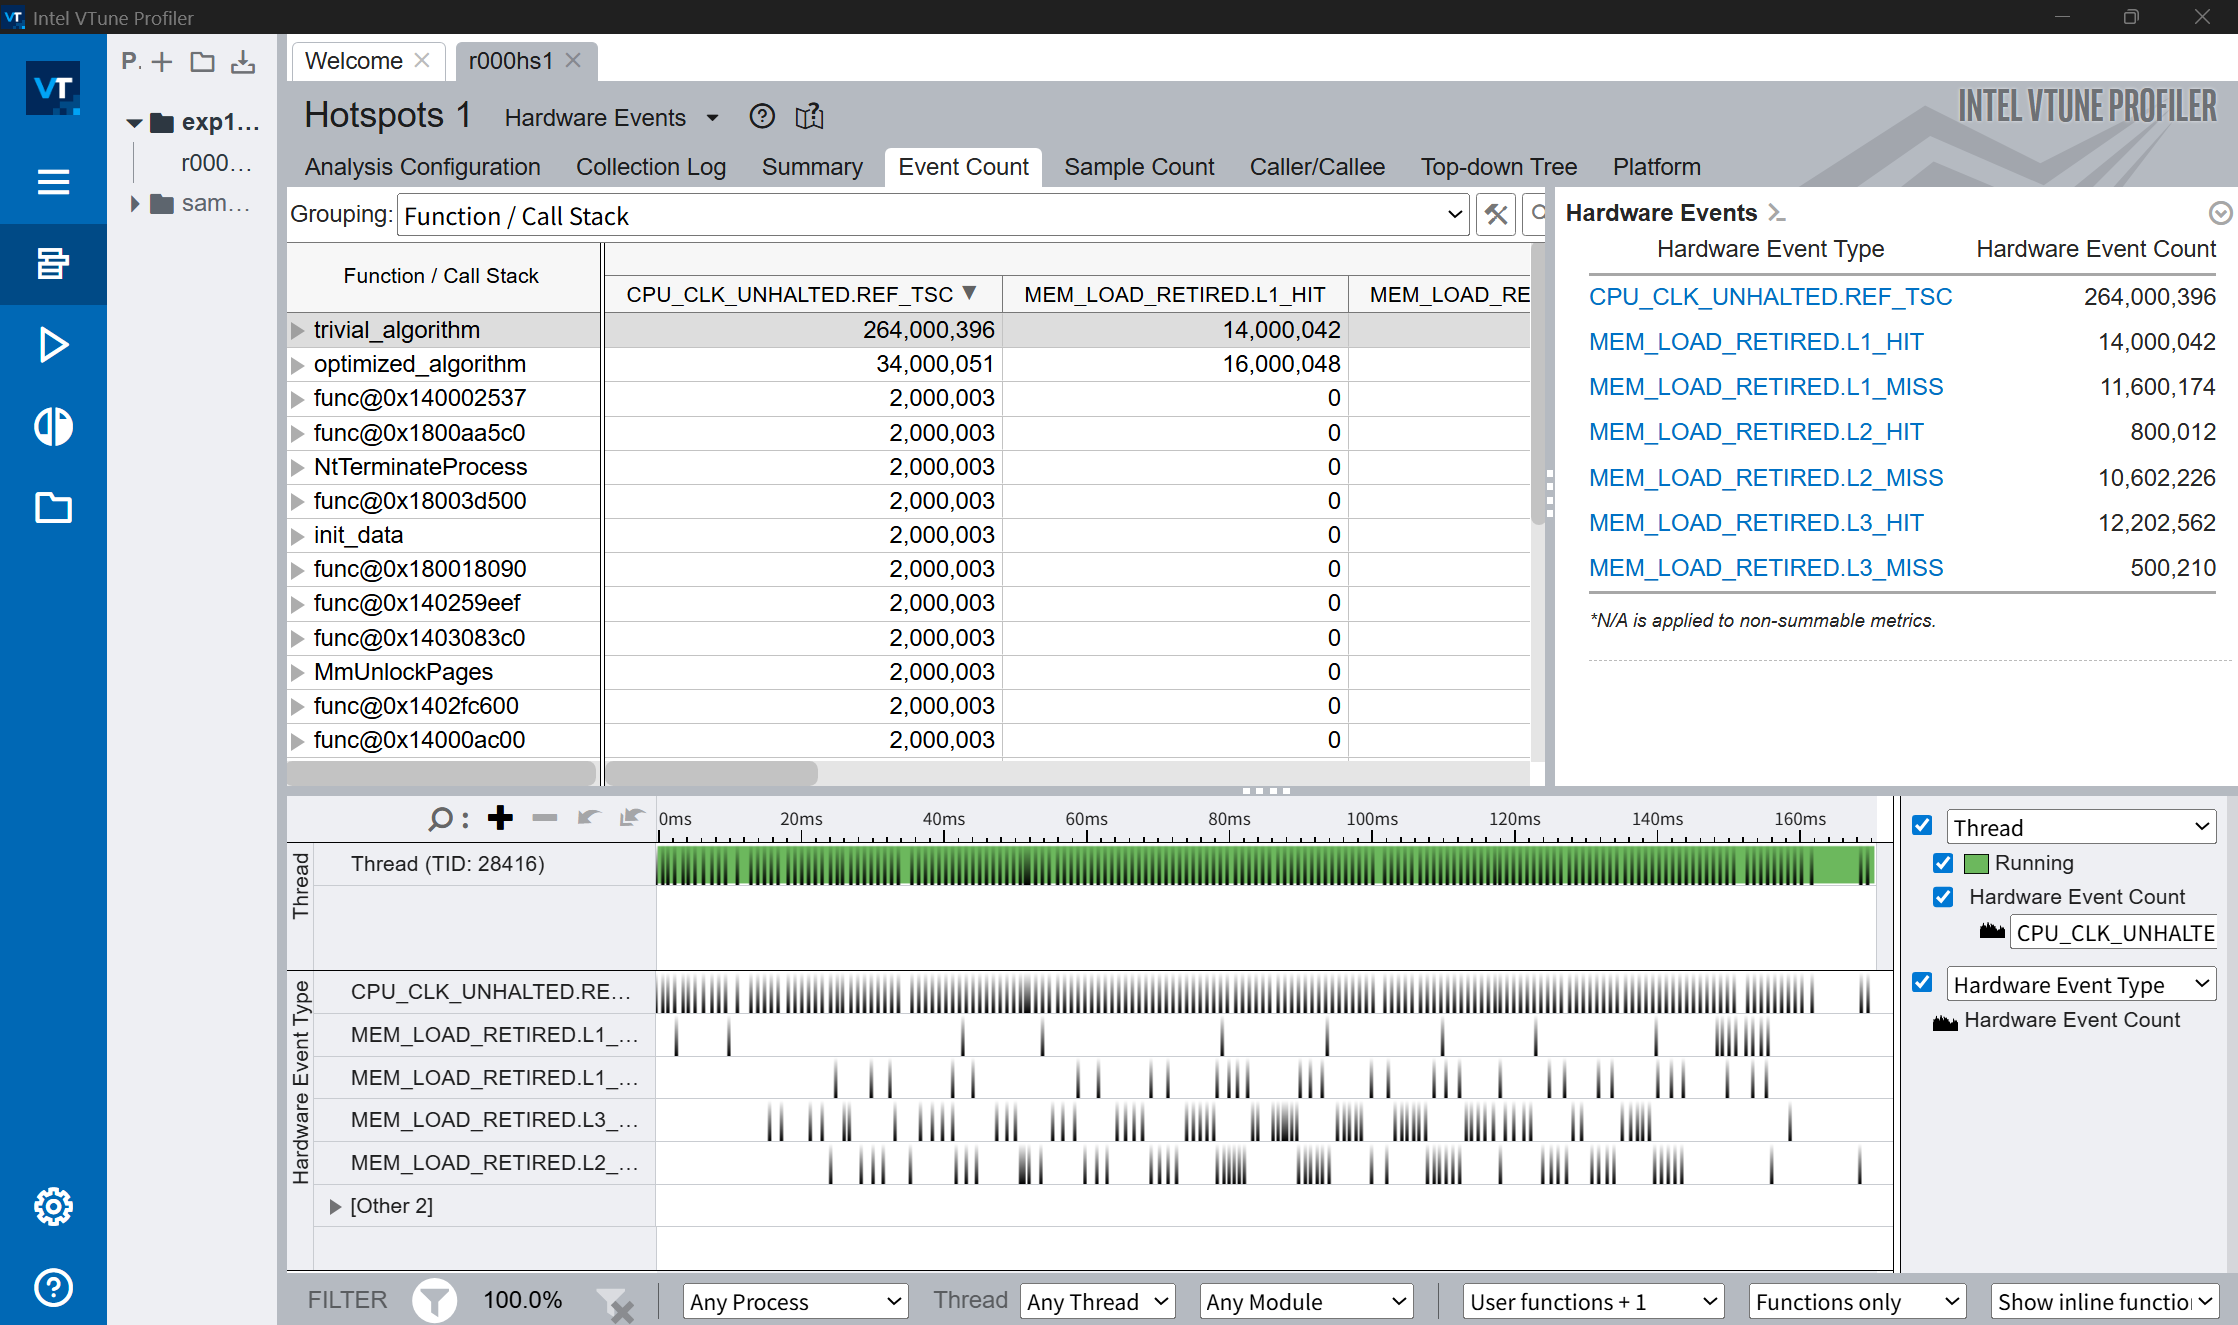
\includegraphics[width=0.8\textwidth]{fig/VTune.png}
\end{figure}

在 x86 平台上使用 Intel VTune Profiler 对实验一进行Hardware
Event-Based Sampling，选取矩阵规模 $n=512$，两种算法各执行 50 次。采样事件包括
六项内存访问相关计数器：\texttt{MEM\_LOAD\_RETIRED.L1/L2/L3\_HIT} 与
\texttt{MEM\_LOAD\_RETIRED.L1/L2/L3\_MISS}。各函数的完整采样结果如表所示。

\begin{table}[!ht]
\centering
\caption{VTune 硬件事件采样结果（$n=512$，\texttt{-O2}）}
\label{tab:vtune}
\begin{tabular}{l r r r r r r}
\toprule
函数 & L1\_HIT & L1\_MISS & L2\_HIT & L2\_MISS & L3\_HIT & L3\_MISS \\
\midrule
\texttt{trivial\_algorithm}   & 14,000,042 & 11,600,174 & 800,012 & 10,602,226 & 12,202,562 & 500,210 \\
\texttt{optimized\_algorithm} & 16,000,048 &  1,200,018 & 1,600,024 &   200,042 &    200,042 &       0 \\
\bottomrule
\end{tabular}
\end{table}

\textbf{L1 miss 率}：平凡算法按列访问，步长为 $512 \times 8 = 4096$ 字节，
每次访问的数据均不在已加载的 cache line 中，L1 miss 率约 45.3\%。优化算法
将循环顺序调整为按行访问，步长 8 字节，加载一条 cache line 后其中 8 个
相邻元素可连续复用，L1 miss 率降至约 7.0\%。

\textbf{L2/L3 穿透}：由于 L1 miss 率高，平凡算法的大量请求继续向下穿透，
L3 miss 达 500,210 次，部分数据需从主存获取。优化算法的 L3 miss 为 0，
所有数据在 L2 层级即可满足，完全避免了访问主存的开销。

\textbf{小结}：优化的核心在于将列访问改为行访问，使 cache line 的空间局部性
得到充分利用，从而将访存层级从主存拉回到 L2，这是两种算法性能差距的根本原因。

% ============================================================
% Lab02 实验二报告正文
% 将本文件内容嵌入主报告的对应 \section 中
% 依赖宏包：minted, booktabs, graphicx, subfigure/subcaption
% ============================================================

\section{体系结构相关实验分析————$n$ 个数求和}

\subsection{实验目的}

通过对 $n$ 个整数求和问题的多种算法实现，理解超标量处理器的指令级并行（ILP）
特性与循环展开优化对程序性能的影响；并以浮点求和为例，
探索累加顺序的改变对计算结果精度的影响。

\subsection{算法实现}

\subsubsection{平凡算法}

\begin{minted}[linenos, frame=lines, framesep=2mm]{cpp}
int sum_naive(int *a, int n) {
    int s = 0;
    for (int i = 0; i < n; i++) s += a[i];
    return s;
}
\end{minted}

\subsubsection{N路循环展开算法}

引入 $N$ 个独立的累加变量，每次循环步进 $N$，同时推进 $N$ 路累加。
$N$ 个独立变量之间不存在数据依赖，处理器可在同一时钟周期内同时发射多条加法指令，
充分利用了超标量。
最终各路部分和通过 \texttt{common\_algo} 归约。
本实验实现了 2、4、8、16、32 路五个版本，以 8 路为例：

\begin{minted}[linenos, frame=lines, framesep=2mm]{cpp}
int sum_unroll8(int *a, int n) {
    int t[8] = {0};
    for (int i = 0; i < n; i += 8) {
        t[0]+=a[i];   t[1]+=a[i+1]; t[2]+=a[i+2]; t[3]+=a[i+3];
        t[4]+=a[i+4]; t[5]+=a[i+5]; t[6]+=a[i+6]; t[7]+=a[i+7];
    }
    return common_algo(t, 8);
}
\end{minted}

\subsubsection{递归算法}

采用二重循环实现两两归并，经 $\log_2 n$ 轮后得到最终结果。

\begin{minted}[linenos, frame=lines, framesep=2mm]{cpp}
int sum_recursive(int *a, int n) {
    for (int m = n; m > 1; m /= 2)
        for (int i = 0; i < m / 2; i++)
            a[i] = a[2*i] + a[2*i+1];
    return a[0];
}
\end{minted}

\subsection{实验过程}

编写测试驱动程序，通过命令行参数指定算法、规模和重复次数，以 \texttt{clock\_gettime(CLOCK\_MONOTONIC)} 计时。

测试规模取 2 的幂，共 10 个规模点：
$n \in \{2^{13}, 2^{14}, 2^{15}, 2^{16}, 2^{17}, 2^{18}, 2^{19}, 2^{20}, 2^{22}, 2^{26}\}$，
涵盖从远小于 L1 Cache 到远超 L3 Cache 的完整范围，同时对小规模配置较多重复次数。
所有性能实验统一采用 \texttt{-O2 -march=native} 编译。

浮点精度探索实验使用 \texttt{float} 类型，数组以 $1/16$ 的概率填入大数（\texttt{1e6f}），
其余填入 \texttt{0.1f}，用以放大累加顺序导致的精度差异。
以 \texttt{double} 精度计算的结果作为参考值，比较各算法的绝对误差。

\subsection{实验结果}

\subsubsection{整数算法性能对比}

\begin{figure}[!ht]
    \centering
    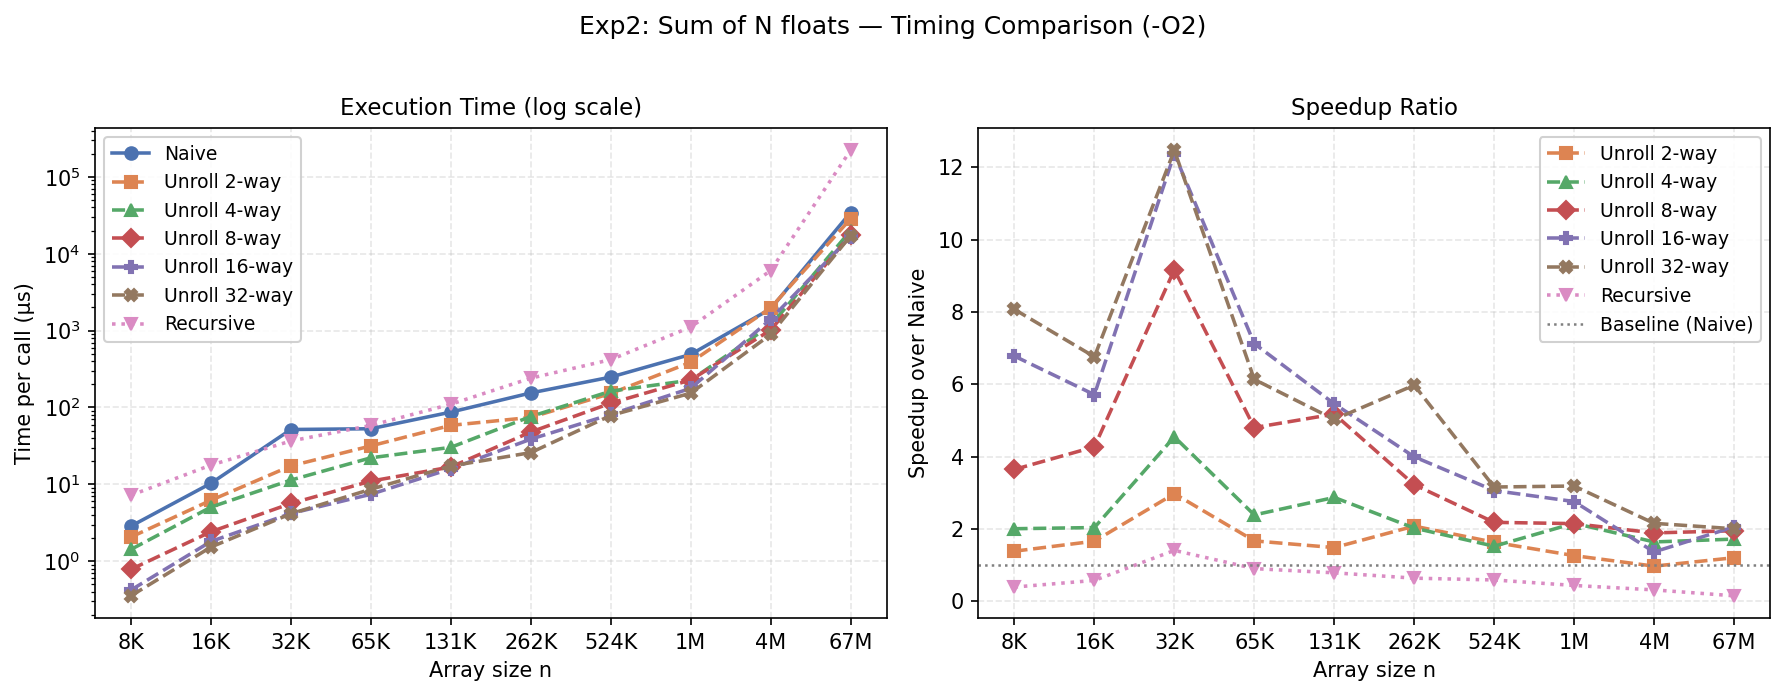
\includegraphics[width=\linewidth]{fig/fig_exp2_time.png}
    \caption{各算法执行时间（\texttt{-O2 -march=native}）}
    \label{fig:exp2_time}
\end{figure}

\begin{table}[!ht]
\centering
\caption{各算法执行时间（$\mu$s/次）及相对 naive 的加速比}
\label{table:exp2_time}
\begin{tabular}{@{}lrrrrrr@{}}
\toprule
$n$ & naive & unroll2 & unroll4 & unroll8 & unroll16 & unroll32 \\
\midrule
$2^{13}$ &  2.86 &  2.06 (1.4x) &  1.42 (2.0x) &  0.78 (3.6x) &  0.42 (6.8x) &  0.35 (8.1x) \\
$2^{15}$ & 51.67 & 17.36 (3.0x) & 11.36 (4.5x) &  5.64 (9.2x) &  4.18 (12.4x) & 4.15 (12.5x) \\
$2^{17}$ & 87.02 & 58.52 (1.5x) & 30.29 (2.9x) & 16.81 (5.2x) & 15.94 (5.5x) & 17.31 (5.0x) \\
$2^{20}$ & 489.53 & 386.86 (1.3x) & 226.69 (2.2x) & 227.72 (2.1x) & 177.41 (2.8x) & 153.53 (3.2x) \\
$2^{26}$ & 34404.65 & 28485.40 (1.2x) & 19981.82 (1.7x) & 17611.52 (2.0x) & 16704.64 (2.1x) & 17140.70 (2.0x) \\
\bottomrule
\end{tabular}
\end{table}

\begin{table}[!ht]
\centering
\caption{递归算法执行时间（$\mu$s/次）}
\label{table:exp2_recursive}
\begin{tabular}{@{}lrrrrrr@{}}
\toprule
$n$ & $2^{13}$ & $2^{15}$ & $2^{17}$ & $2^{20}$ & $2^{22}$ & $2^{26}$ \\
\midrule
recursive & 7.21 & 36.65 & 110.15 & 1111.06 & 6034.30 & 222080.81 \\
naive      & 2.86 & 51.67 &  87.02 &  489.53 & 1922.46 &  34404.65 \\
比值       & 2.5x慢 & 1.4x快 & 1.3x慢 & 2.3x慢 & 3.1x慢 & 6.5x慢 \\
\bottomrule
\end{tabular}
\end{table}

\subsubsection{浮点精度探索}

\begin{table}[!ht]
\centering
\caption{各算法浮点求和结果与参考值（\texttt{double} 精度）的绝对误差}
\label{table:exp2_float}
\begin{tabular}{@{}lrrrrrrr@{}}
\toprule
$n$ & naive & unroll2 & unroll4 & unroll8 & unroll16 & unroll32 & 参考值(double) \\
\midrule
$2^5$   & 0.75   & 0.38   & 0.00   & 0.12   & 0.75   & 0.75   & 2000003 \\
$2^{10}$ & 92     & 44     & 24     & 12     & 24     & 24     & 64000096 \\
$2^{13}$ & 768    & 352    & 192    & 96     & 192    & 192    & 512000768 \\
$2^{16}$ & 199424 & 196096 & 194816 & 194048 & 191744 & 122880 & 4096006144 \\
$2^{19}$ & 5664768 & 5638144 & 5627904 & 5621760 & 5603328 & 6033408 & 32768049152 \\
$2^{22}$ & 138117120 & 137904128 & 137822208 & 137773056 & 137625600 & 124370944 & 262144393216 \\
\bottomrule
\end{tabular}
\end{table}

\subsection{数据分析}

\subsubsection{整数算法性能对比}
\begin{enumerate}
    \item 展开路数越多，小到中规模的加速效果越显著:
    在 $n=2^{13}$（数据完全在 L1 Cache 内）时，unroll32 相对 naive 的加速比达到 8 倍，
unroll16 也有近 7 倍，而 unroll2 仅有 1.4 倍。
说明在内存访问不构成瓶颈时，独立累加变量数目越多，
超标量流水线的利用率越高，收益越明显。

   \item 当 $n=2^{26}$也就是数据远超 L3 Cache时，即使是 unroll32 相对 naive 的加速比也仅约 2 倍。
此时数组的每次访问都可能触发 Cache Miss，处理器执行单元大部分时间在等待内存数据，
多路并行的优势被访存延迟所掩盖，内存带宽成为共同的瓶颈。
\end{enumerate}


\subsubsection{进阶任务：浮点精度探索}

浮点加法不满足结合律，累加顺序不同会导致中间结果不同，
进而引入不同的舍入误差。表~\ref{table:exp2_float} 展示了这一现象。
\begin{enumerate}
    \item \textbf{误差随规模增大而快速累积。}
在 $n=2^5$ 时，各算法误差在 1 以下，可忽略不计；
而到 $n=2^{22}$ 时，误差已达到 $10^8$ 量级，
相对误差约为 0.05\%。这是因为每次加法操作都可能引入约半个 ULP 的舍入误差，
误差随操作次数大致线性累积。
    \item  \textbf{各算法之间的误差规律：}
在中小规模时，unroll8 的误差最小，这与其将数据切分为 8 个独立的较小部分和有关，
每路累加的数值范围更小，相对舍入误差更低。
naive 的误差则普遍偏大，因为它将所有元素串行累加到同一个变量中，
随着该变量不断增大，后续的小数相加时精度损失就更加严重。
\end{enumerate}





\subsection{进阶任务：使用VTune进行Profiling}
\subsubsection{VTune 微架构分析}

使用 Intel VTune Profiler 对三个代表性算法进行 Microarchitecture Exploration 分析，
测试规模 $n=2^{20}$，重复 5000 次。关键指标汇总见表~\ref{table:vtune}。

\begin{table}[H]
\centering
\label{table:vtune}
\begin{tabular}{@{}lrrrr@{}}
\toprule
指标 & naive & unroll8 & unroll32 & recursive \\
\midrule
CPI                   & 0.540  & 0.378  & 1.064  & 0.364  \\
IPC                   & 1.853  & 2.645  & 0.939  & 2.751  \\
Retiring \%           & 18.8\% & 82.5\% & 16.1\% & 39.7\% \\
Backend Bound \%      & 50.0\% & 50.0\% & 90.3\% & 49.0\% \\
\quad Memory Bound \% & 17.6\% & 12.5\% & 45.2\% & 34.4\% \\
\quad Core Bound \%   & 32.4\% & 37.5\% & 45.2\% & 14.6\% \\
L1D Miss Stall（占周期）& 34.7\% & 13.9\% & 50.9\% & 22.9\% \\
L3 Miss Stall（占周期）&  3.7\% &  1.7\% &  1.8\% & 10.8\% \\
L3 Miss 率            &  0.0\% &  0.0\% &  0.0\% & 11.8\% \\
总 Slots（$\times 10^9$）& 8.84 & 4.16 & 8.06 & 74.88 \\
Elapsed（ms）         & $\approx$900 & 909 & 1078 & 8304  \\
\bottomrule
\end{tabular}
\end{table}

由数据可知，unroll8的有效工作比例最高， Retiring 达到 82.5\%，
说明处理器超过五分之四的时钟周期都在做有效工作。
与 naive 相比，CPI 从 0.540 降至 0.378，
IPC 从 1.853 提升至 2.645。
更关键的是，unroll8 完成相同工作所消耗的总时钟槽数（Slots）只有 naive 的 47\%
，说明其资源利用率从根本上得到了改善。
同时，和前面的测试数据相印证，recursive 每个归并步骤需要读取和写回数组元素，
而且随着归并层数增加，访问跨度呈指数增长，导致大量 L3 Cache Miss，naive 和 unroll 均为 0\%
造成总执行时间比naive的算法更长。

\newpage
\bibliographystyle{plain}
\bibliography{reference.bib} 

\end{document}